
\begin{enumerate}[\Large\bfseries 1.]

%--------------------1.
\item \textbf{COEFICIENTE BINOMIAL} (Capítulo 2, problema 3. Michael Spivak, Calculo Infinitesimal. )\\\\

    \begin{enumerate}[\bfseries a)]

	%----------a.
	\item Si $0\leq k \leq n,$ se define el coeficiente binomial $\displaystyle \binom{n}{k}$ por
	    $$\binom{n}{k} = \dfrac{n!}{k!(n-k)!} = \dfrac{n(n-1) \cdots (n-k+1)}{k!}, \quad si \; k\neq 0, n$$\\\\

	%----------b)
	\item \textbf{Código fuente.}\\ 
	    
	    \lstinputlisting[language=Python]{python/tareas_mat/week2/coe_binom.py}
	    \vspace{3cm}
	
	%----------c)
	\item \textbf{Prueba de la ejecución del programa}.\\
	    \begin{center}
		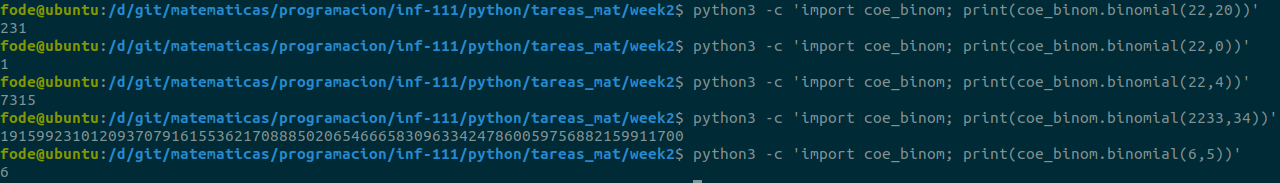
\includegraphics[scale=.35]{imagenes/tareas_mat/week2/coe_binom.png}
	    \end{center}

    \end{enumerate}

\newpage


%--------------------2.
\item \textbf{NÚMERO NATURAL PAR O IMPAR} (Capítulo 2, problema 8. Michael Spivak, Calculo Infinitesimal. )\\\\

    \begin{enumerate}[\bfseries a)]

	%----------a.
	\item Demostrar que todo número natural es o par o impar.\\\\
	    Demostración.- \; Asumimos que $n$ es impar o par, entonces debemos probar que $n+1$ también, es o bien impar o bien par.\\ 
	    Sea $n$ par entonces $n=2k$ para algún $k$. Así $n+1=2k+1$  y por definición vemos que es impar.\\
	    Luego sea $n$ impar, entonces $n=2k+1$ para algún $k$.  Por lo tanto $n+1=2k+1+1 = 2k +2 = 2(k+1)$. Así en cualquiera de los dos casos, $n+1$ es o bien par o impar. \\\\  

	%----------b)
	\item \textbf{Código fuente.}\\ 
	    
	    \lstinputlisting[language=Python]{python/tareas_mat/week2/par_impar.py}
	    \vspace{1cm}
	
	%----------c)
	\item \textbf{Prueba de la ejecución del programa}.\\
	    \begin{center}
		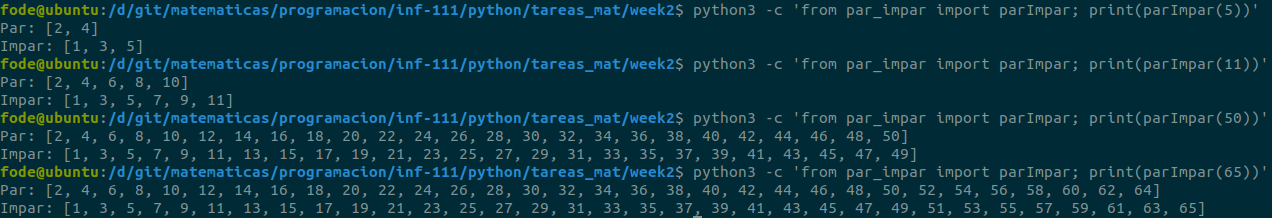
\includegraphics[scale=.35]{imagenes/tareas_mat/week2/par_impar.png}
	    \end{center}

    \end{enumerate}

\newpage

%--------------------3.
\item \textbf{DESIGUALDAD DE BERNOULLI} (Capítulo 2, problema 19. Michael Spivak, Calculo Infinitesimal. )\\\\

    \begin{enumerate}[\bfseries a)]

	%----------a.
	\item Demostrar la desigualdad de Bernoulli: Si $h>-1$, entonces $$(1+h)^n \geq 1 + nh$$
      ¿Por qué es esto trivial si $h>0$?\\\\
      Demostración.-\; Si $n=1$, entonces $(1+h)^n=1+nh$. Supóngase que $(1+h)^n \geq 1+nh.$ Entonces $(1+h)^n+1=(1+h)(1+h)^n \geq (1+h)(1+nh)$, ya que $1+h>0$ luego $1+(n+1)h+nh^2\geq 1+(n+1)h$\\
      Para $h>0$, la igualdad se sigue directamente del teorema del binomio, ya que todos los demás términos que aparecer en el desarrollo de $(1+h)^n$ son positivos.\\\\ 

	%----------b)
	\item \textbf{Código fuente.}\\ 
	    
	    \lstinputlisting[language=Python]{python/tareas_mat/week2/bernoulli.py}
	    \vspace{1cm}
	
	%----------c)
	\item \textbf{Prueba de la ejecución del programa}.\\
	    \begin{center}
		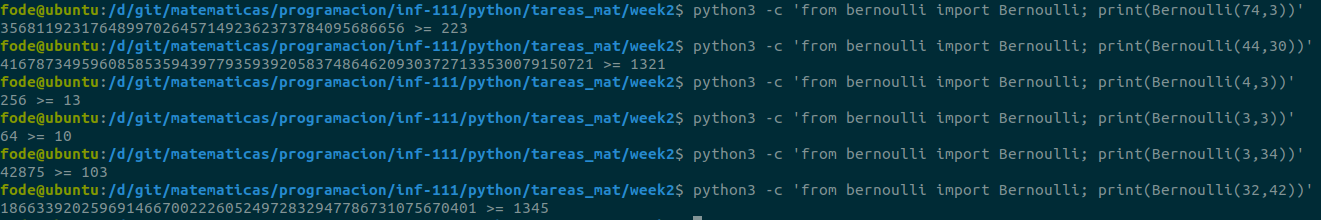
\includegraphics[scale=.35]{imagenes/tareas_mat/week2/bernoulli.png}
	    \end{center}

    \end{enumerate}

\newpage

%--------------------3.
\item \textbf{SUCESIÓN DE FIBONACCI} (Capítulo 2, problema 20. Michael Spivak, Calculo Infinitesimal. )\\\\

    \begin{enumerate}[\bfseries a)]

	%----------a.
	\item La sucesión de Fibonacci $a_1,a_2,a_3,...$ se define como sigue:
      \begin{center}
	 \begin{tabular}{rcll}
	    $a_1$ & $=$ & $1,$ & \\
	    $a_2$ & $=$ & $1,$ & \\
	    $a_n$ & $=$ & $a_{n-1} + a_{n-2}$ & para $n \geq 3$\\
	 \end{tabular}
      \end{center}
      Esta sucesión, cuyos primeros términos son $1,1,2,3,5,8,...,$ fue descubierta por Fibonacci (1175-1250, aprox.) en relación con un problema de conejos. Fibonacci supuso que una pareja de conejos criaba una nueva pareja cada mes y que después de dos meses cada nueva pareja se comportaba del mismo modo. El número $a_n$ de parejas nacidas en el n-ésimo mes es $n_{n-1} + a_{n-2}$, puesto que nace una pareja por cada pareja nacida en el mes anterior, y además, cad pareja nacida hace dos meses produce ahora una nueva pareja. Es verdaderamente asombroso el número de resultados interesantes relacionados con esta sucesión, hasta el punto de existir una Asociación de Fibonacci que publica una revista, the Fibonacci Quarterly.\\
      Demostrar que $$a_n = \dfrac{\left( \dfrac{1+\sqrt{5}}{2} \right)^n - \left( \dfrac{1-\sqrt{5}}{2} \right)^n}{\sqrt{5}}$$\\
      Demostración.- \; Al ser $$\dfrac{\left( \dfrac{1+\sqrt{5}}{2} \right)^1 - \left( \dfrac{1-\sqrt{5}}{2} \right)^1}{\sqrt{5}}=\dfrac{\sqrt{5}}{\sqrt{5}}=1$$
      La fórmula es válida para $n=1$ y también se cumple para $n=1$. Supóngase que es válida para todo $k<n,$ donde $n\geq 3.$ En tal caso es válida en particular para $n-1$ y para $n-2$, luego por hipótesis
      \begin{center}
	 \begin{tabular}{rcl}
	    $a_n$ & $=$ & $a_{n-1} + a_{n-2}$\\\\
		  & $=$ & $\dfrac{\left( \dfrac{1+\sqrt{5}}{2} \right)^{n-2} - \left( \dfrac{1-\sqrt{5}}{2} \right)^{n-2} + \left( \dfrac{1+\sqrt{5}}{2} \right)^{n-1} - \left( \dfrac{1-\sqrt{5}}{2} \right)^{n-1}}{\sqrt{5}}$\\\\
		  & $=$ & $\dfrac{\left( \dfrac{1+\sqrt{5}}{2}\right)^{n-2} \left( \dfrac{1+\sqrt{5}}{2} \right) - \left( 1 - \dfrac{1-\sqrt{5}}{2} \right)^{n-2} \left( 1 - \dfrac{1- \sqrt{5}}{2} \right)}{\sqrt{5}}$\\\\
		  & $=$ & $\dfrac{\left( \dfrac{1+\sqrt{5}}{2} \right)^{n-2} \left( \dfrac{1+\sqrt{5}}{2}\right)^2 - \left( 1 - \dfrac{1-\sqrt{5}}{2} \right)^{n-2} \left( 1 - \dfrac{1-\sqrt{5}}{2} \right)^2}{\sqrt{5}}$\\\\
	       & $=$ & $\dfrac{\left( \dfrac{1+\sqrt{5}}{2} \right)^n - \left( \dfrac{1-\sqrt{5}}{2} \right)^n}{\sqrt{5}}$\\\\
	 \end{tabular}
      \end{center}
      \newpage

	%----------b)
	\item \textbf{Código fuente.}\\ 
	    
	    \lstinputlisting[language=Python]{python/tareas_mat/week2/fibo.py}
	    \vspace{1cm}
	
	%----------c)
	\item \textbf{Prueba de la ejecución del programa}.\\
	    \begin{center}
		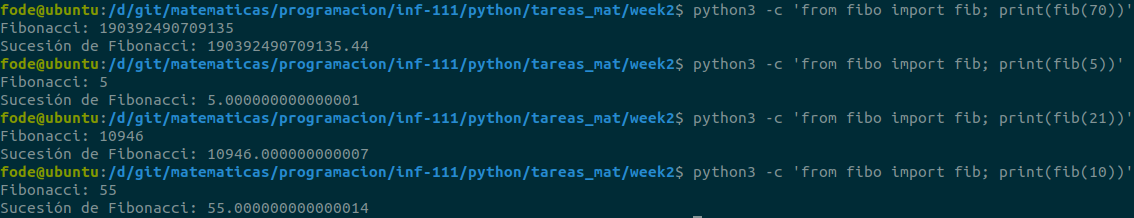
\includegraphics[scale=.35]{imagenes/tareas_mat/week2/fibo.png}
	    \end{center}

    \end{enumerate}

\newpage


%--------------------4.
\item \textbf{DESIGUALDAD DE SCHWARZ} (Capítulo 2, problema 21. Michael Spivak, Calculo Infinitesimal. )\\\\

    \begin{enumerate}[\bfseries a)]

	%----------a.
	\item La desigualdad de Schwarz (problema 1-19) tiene en realidad una forma más general: $$\displaystyle\sum_{i=1}^n x_1 y_1 \leq \sqrt{\sum_{i=1}^n x_i^2} \sqrt{\sum_{i=1}^n y_i^2}$$
      Dar de esto tres demostraciones, análogas a las tres demostraciones del problema 1-19\\\\
      Demostración.-\; 
      \begin{enumerate}[\bfseries i)]
	 \item Como antes, la demostración es trivial si para todo $y_i=0$ o si hay algún numero $\lambda$ con $x_i=\lambda y_i$ para todo $i$. Es decir, 
	    \begin{center} 
	       \begin{tabular}{rcl}
		  $0$ & $<$ & $\sum\limits_{i=1}n (\lambda y_i - x_i)^2$\\\\
		   & $=$ & $\lambda \left( \sum\limits_{i=1}^n y_i^2 \right) -2 \lambda \left( \sum\limits_{i=1}^n x_i y_i\right) + \sum\limits_{i=1}^n x_i^2$\\\\
	       \end{tabular}
	       así por el problema 1-18 queda demostrado. 
	    \end{center}
	 \item Usando $2xy \leq x^2 + y^2$ con 
            $$x=\dfrac{x_i}{\sqrt{\sum\limits_{i=1}^n x_i^2}}, \,\,\,\, y=\dfrac{y_i}{\sqrt{\sum\limits_{i=1}^n y_i^2}}$$
            obtenemos, 
            $$\dfrac{2x_iy_1}{\sqrt{\sum\limits_{i=1}^n x_i^2} \sqrt{\sum\limits_{i=1}^n y_i^2}} \leq \dfrac{x_i^2}{\sum\limits_{i=1}^n x_i^2} + \dfrac{y_i^2}{\sum\limits_{i=1}^n y_i^2} \,\,\,\, (1)$$
            luego
            $$\dfrac{\sum\limits_{i=1}^n 2x_iy_i}{\sqrt{\sum\limits_{i=1}^n x_i^2} \sqrt{\sum\limits_{i=1}^n y_i^2}} \leq \dfrac{\sum\limits_{i=1}^n x_i^2}{\sum\limits_{i=1}^n x_i^2} + \dfrac{\sum\limits_{i=1}^n y_i^2}{\sum\limits_{i=1}^n y_i^2}=2$$
            Nuevamente, la igualdad se cumple solo si se cumple en $(1)$ para todo $i$, lo que significa que, 
            $$\dfrac{x_i}{\sqrt{\sum\limits_{i=1}^n x_i^2}} = \dfrac{y_i}{\sqrt{\sum\limits_{i=1}^n y_i^2}}$$
            para todo $i$. Si todo $y_i$ es distinto de $0$. Esto significa que $x_i=\lambda y_i$ para 
            $$\lambda = \dfrac{\sqrt{\sum\limits_{i=1}^n x_i^2}}{\sqrt{\sum\limits_{i=1}^n y_i^2}}$$
         \item La demostración depende de la siguiente igualdad:
            $$\sum\limits_{i=1}^n x_i^2 \cdot \sum\limits_{i=1}^n y_i^2 = \left( \sum\limits_{i=1}^n x_iy_i \right)^n + \sum\limits_{i<j} (x_i y_j -x_j y_i)^2$$
            al verificar esta igualdad notamos que,
            $$\sum\limits_{i=1}x_i^2 \cdot \sum\limits_{i=1}^n y_i^2 = \sum\limits_{i=1}^n x_i^2 y_i^2 + \sum\limits_{i\neq j} x_i2 y_j^2$$
             y por lo tanto,
             $$\left( \sum\limits_{i=1}^n x_i y_i \right)^2 = \sum\limits_{i=1}^n (x_i y_i)^2 + \sum\limits_{i\neq j} x_i y_i x_j y_j$$
             La diferencia es
             \begin{center} 
                \begin{tabular}{rlc}
                   $\sum\limits_{i \neq j} (x_i^2 y_j^2 - x_i y_i x_j y_j)$ & $=$ & $2 \sum\limits_{i<j} (2_i^2 y_j^2 + x_j^2 y_i^2 - x_i y_i x_j y_j)$\\\\
                      & $=$ & $2 \sum\limits_{i<j} (x_i y_j - x_j y_i)^2$\\\\
                \end{tabular}
             \end{center}
             Si la igualdad se cumple en la desigualdad de Schwarz, para todo $x_iy_j = x_j y_i$. Si algún $y_i \neq 0$ y $y_i \neq 0$, luego $x_i=\dfrac{x_1}{y_1}y_i$ para todo $i$, así tenemos que $\lambda = \dfrac{x_1}{y_1}$\\\\
      \end{enumerate} 

	%----------b)
	\item \textbf{Código fuente.}\\ 
	    
	    \lstinputlisting[language=Python]{python/tareas_mat/week2/schwarz.py}
	    \vspace{1cm}
	
	%----------c)
	\item \textbf{Prueba de la ejecución del programa}.\\
	    \begin{center}
		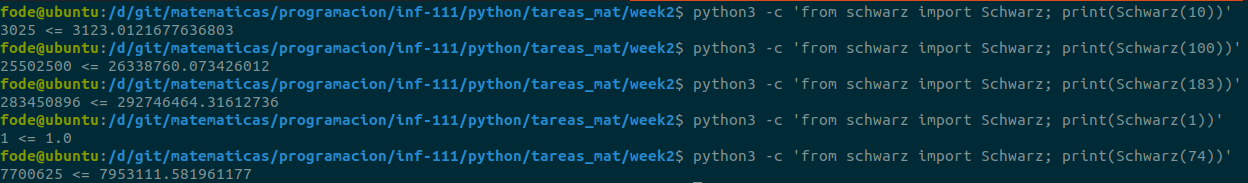
\includegraphics[scale=.35]{imagenes/tareas_mat/week2/schwarz.png}
	    \end{center}

    \end{enumerate}

\newpage



\end{enumerate}
